%0       1         2         3         4         5         6         7         8
%2345678901234567890123456789012345678901234567890123456789012345678901234567890

\documentclass[10pt]{article}


% INCLUDE DEVELOPMENT TEXT

\newcommand{\devel}[1]{\textbf{#1}}

% EXCLUDE DEVELOPMENT TEXT

% \newcommand{\devel}[1]{}


%=======================================================================
% Document layout
%=======================================================================

\setlength{\topmargin}{0.0in}
\setlength{\oddsidemargin}{0.0in}
\setlength{\evensidemargin}{0.0in}
\setlength{\textwidth}{6.0in}
\setlength{\textheight}{9.0in}

%=======================================================================
% Packages
%=======================================================================

\usepackage{wasysym}
\usepackage{epsfig}
\usepackage{url}

%=======================================================================
% Commands
%=======================================================================

\newcommand{\cello}{\textsf{Cello}}
\newcommand{\enzo}{\textsf{Enzo}}
\newcommand{\lcaperf}{\textsf{lcaperf}}
\newcommand{\lcatest}{\textsf{lcatest}}

\newcommand{\code}[1]{\textsf{#1}}

\newcommand{\note}[1]{\devel{\eighthnote\ \textit{#1} \\}}
\newcommand{\pargraph}[1]{\devel{\P\ \textbf{#1} \\}}

\newcommand{\todo}{\devel{$\circ$}}
\newcommand{\done}{\devel{$\bullet$}}
\newcommand{\halfdone}{\devel{\textcolor{gray}{$\bullet$}}}

\newcommand{\PROJECT}{\cello}

\newcommand{\TITLE}[3]{
\title{ {\huge \PROJECT\ #1}  \\ \vspace{0.1in}
     {\small Document Version: \textbf{#3}} \vspace{-0.1in}
    }
\author{      #2 \\
        Laboratory for Computational Astrophysics\\
        University of California, San Diego}
\maketitle}

%=======================================================================


%==================================================================
% Margins and spacing
%==================================================================

\begin{document}

%=======================================================================
\TITLE{\hypre\ SAMR Linear Solver}
      {James Bordner}
      {in preparation}
%=======================================================================

\tableofcontents
%======================================================================
\section{Overview}
%======================================================================

   \hypresolve\ will be used as a testbed for experimenting with the
   parallel solution of linear systems arising from self-gravity
   (Poisson equation) and radiation transfer algorithms (diffusion
   equation) defined on distributed SAMR hierarchies.  The purpose of
   this document is to specify the requirements, describe the design
   and implementation, and present test results for \hypresolve.

   We decompose the problem into two components: problem generation
   (\code{hypre-init}), and problem solution (\code{hypre-solve}).
   \code{hypre-init} takes as input parameters describing the problem
   characteristics in general terms, such as bounds on grid sizes,
   number of processors, description of how to distribute point
   masses, etc.  The output is a file of parameters that specify the
   exact problem to solve, including grid locations, sizes, levels,
   point mass locations, etc.  The file output by \code{hypre-init}
   can be subsequently read by \code{hypre-solve}.  \code{hypre-solve}
   calls \hypre\ to generate and solve a distributed linear system,
   and the solution, performance information, solver efficiency
   information, etc., are output.

%======================================================================
\section{Roadmap and Milestones}
%======================================================================


\begin{description}
\item[Driver: ] \code{hypre-solve} (H), \enzo\ (E)
\item[Equation: ] Poisson (P), diffusion equation (D)
\item[Datastructure: ] Unigrid (U), AMR (A)
\item[AMR refinement: ] $R=2$ (2), $R=2^k$ (2k), arbitrary $R$ (*)
\item[AMR discretization: ] $D=1$, $D=3$, $D=4$, $D=6$
\end{description}

\begin{tabular}{cl|cc|cc|cc|ccc|ccc}
Done & \multicolumn{1}{c}{Description} & H&E & P&D & U&A & 2&[2k]&[*] & C&[L]&[Q] \\ \hline
\multicolumn{2}{l|}{Basic Poisson} &&&&&&&&& \\
\done & Unigrid Poisson equation & \done&\todo & \done&\todo & \done&\todo & \done&\todo&\todo & \done&\todo&\todo \\
\todo &AMR Poisson equation  & \done&\todo & \done&\todo & \todo&\done & \done&\todo&\todo & \done&\todo&\todo \\ \hline
\multicolumn{2}{l|}{Basic diffusion} &&&&&&&&& \\
\todo &Unigrid Diffusion equation& \done&\todo & \todo&\done& \done&\todo & \done&\todo&\todo & \done&\todo&\todo  \\
\todo  &AMR Diffusion equation& \done&\todo & \todo&\done& \todo&\done & \done&\todo&\todo & \done&\todo&\todo \\  \hline
\multicolumn{2}{l|}{higher-order discretizations} &&&&&&&&& \\
\todo  &piecewise linear Poisson & \done&\todo & \done&\todo & \todo&\done & \done&\todo&\todo & \todo&\done&\todo \\
\todo  &  piecewise linear Diffusion & \done&\todo & \todo&\done& \todo&\done & \done&\todo&\todo & \todo&\done&\todo \\  
\todo &piecewise quadratic Poisson & \done&\todo & \done&\todo& \todo&\done & \done&\todo&\todo & \todo&\todo&\done \\  
\todo &piecewise quadratic Diffusion & \done&\todo & \todo&\done& \todo&\done & \done&\todo&\todo & \todo&\todo&\done \\  \hline
\multicolumn{2}{l|}{more general refinement factors} &&&&&&&&& \\
\todo &$2^k$ refinement factors  & \done&\todo & \todo&\done& \todo&\done & \todo&\done&\todo & \done&\todo&\todo\\
\todo & arbitrary refinement factors & \done&\todo & \todo&\done& \todo&\done & \todo&\todo&\done & \done&\todo&\todo \\  \hline
\multicolumn{2}{l|}{\enzo\ port} &&&&&&&&& \\
\todo &port to \enzo & \todo&\done & \fade&\fade& \fade&\fade & \fade&\fade&\fade & \fade&\fade&\fade
\end{tabular}

%======================================================================
\section{\code{hypre-init}} \label{ss:hypre-init}
%======================================================================

%----------------------------------------------------------------------
\subsection{Input}
%----------------------------------------------------------------------

\begin{tabbing}
xxxxx\=xxxxxxxxxxxxxxxxxxxxxxxx\=\kill
\> \todo\ \code{dimension} \> \code{\textit{int dimension}} \\
\> \todo\ \code{particle\_position\_clumpiness}  \\
\> \todo\ \code{particle\_mass\_clumpiness} \\
\> \todo\ \code{particle\_mass\_average} \\
\> \todo\ \code{sphere} \> \code{\textit{Scalar mass}, \textit{Scalar radius}, \textit{Scalar*3 center}} \\
\> \todo\  \code{domain\_extents} \\
\> \todo\  \code{processor\_grid} \\
\> \todo\  \code{levels} \\
\end{tabbing}



%=======================================================================
\section{\code{hypre-solve}}  \label{ss:hypre-solve}
%=======================================================================

%----------------------------------------------------------------------
\subsection{Input}
%----------------------------------------------------------------------

The following table lists the input parameters to \code{hypre-solve}.

\begin{tabbing}
xxxxx\=xxxxx\=xxxxxxxxxxx\=\kill
\> \done\ \code{dimension} \icode{dimension} \\
\>\> \icode{dimension}:    \> \code{int}, $1 \le $ \icode{dimension} $\le 3$
\end{tabbing}
\begin{tabbing}
xxxxx\=xxxxx\=xxxxxxxxxxx\=\kill
\> \done\ \code{domain} \icode{dimension} \icode{vertex-lower} \icode{vertex-upper} \\
\>\> \icode{dimension}:    \> \code{int}, $1 \le $ \icode{dimension} $\le 3$ \\
\>\> \icode{vertex-lower}: \> \code{Scalar*3}  \\
\>\> \icode{vertex-upper}: \> \code{Scalar*3}
\end{tabbing}
\begin{tabbing}
xxxxx\=xxxxx\=xxxxxxxxxxx\=\kill
\> \todo\ \code{sphere} \icode{mass} \icode{radius} \icode{center} \\
\> \> \icode{mass}:        \> \code{Scalar}  \\
\> \> \icode{radius}:      \> \code{Scalar}  \\
\> \> \icode{center}       \> \code{Scalar*3}
\end{tabbing}
\begin{tabbing}
xxxxx\=xxxxx\=xxxxxxxxxxx\=\kill
\> \done\ \code{point} \icode{mass} \icode{position} \\
\> \> \icode{mass}:        \> \code{Scalar}  \\
\> \> \icode{position}     \> \code{Scalar*3}
\end{tabbing}
\begin{tabbing}
xxxxx\=xxxxx\=xxxxxxxxxxx\=\kill
\> \done\ \code{grid} \icode{id} \icode{parent-id} \icode{processor} \icode{vertex-lower} \icode{vertex-upper} \icode{index-lower} \icode{zone-count}\\
\> \> \icode{id}:          \> \code{int}  \\
\> \> \icode{parent-id}:   \> \code{int}  \\
\> \> \icode{processor}:   \> \code{int}  \\
\> \> \icode{vertex-lower}:\> \code{Scalar}  \\
\> \> \icode{vertex-upper}:\> \code{Scalar}  \\
\> \> \icode{index-lower}: \> \code{int*3}  \\
\> \> \icode{zone-count}:  \> \code{int*3}
\end{tabbing}
\begin{tabbing}
xxxxx\=xxxxx\=xxxxxxxxxxx\=\kill
\> \todo\ \code{discret} \icode{discret} \\
\> \> \icode{discret}:     \> \code{int} $\in \{\code{"constant"},\code{"linear"},\code{"bilinear"},\code{"quadratic"}\}$
\end{tabbing}
\begin{tabbing}
xxxxx\=xxxxx\=xxxxxxxxxxx\=\kill
\> \done\ \code{solver}  \icode{solver} \\
\> \> \icode{solver}:     \> \code{string} $\in$ \{ ``\code{fac}'', ``\code{pfmg}'', ``\code{bicgstab}'' \}
\end{tabbing}
\begin{tabbing}
xxxxx\=xxxxx\=xxxxxxxxxxx\=\kill
\> \done\ \code{solver\_maxit}  \icode{iterations}
\end{tabbing}
\begin{tabbing}
xxxxx\=xxxxx\=xxxxxxxxxxx\=\kill
\> \done\ \code{solver\_restol}  \icode{tolerance}
\end{tabbing}


%----------------------------------------------------------------------
\subsection{Output}
%----------------------------------------------------------------------

The output of \code{hypre-solve} is a file containing the following:

\begin{tabbing}
xxxxx\=xxxxxxxxxxxxxx\=\kill
\> \todo\ \code{flops-balance} \>    \textit{Load balance efficiency with respect to flops}\\
\> \todo\ \code{flops-proc-avg} \> \textit{Average flop counts over processors} \\
\> \todo\ \code{flops-proc-max} \> \textit{Maximum flop counts over processors} \\
\> \todo\ \code{flops-total} \> \textit{Number of floating point operations} \\
\> \todo\ \code{mem-balance} \>    \textit{Load balance efficiency with respect to memory}\\
\> \todo\ \code{mem-proc-avg} \> \textit{Average memory usage over processors} \\
\> \todo\ \code{mem-proc-max} \>    \textit{Maximum memory usage over processors} \\
\> \todo\ \code{mem-total} \> \textit{Amount of memory used} \\
\> \todo\ \code{procs-total} \> \textit{Number of processors} \\
\> \todo\ \code{time-total} \>  \textit{Time to solution}
\end{tabbing}



%-----------------------------------------------------------------------
\subsection{Functions} \label{ss:design}
%-----------------------------------------------------------------------

The \code{main()} function is in \code{hypre-solve.cpp}.  The main
function begins by reading in the input file, and initializing its
representation of the AMR hierarchy.  Next it calls \hypre\
to have it generate its internal representation of 
the hierarchy, stencil, graph, and linear system.  Then it
calls \hypre\ to solve the linear system, and finally it calls
a function to evaluate evaluate the solution and output 
information about the success of the solve.  Classes \code{problem},
\code{hierarchy}, and \code{hypre} are used to organize the functions.
The high-level  calling code structure is shown below.

\begin{tabbing}
xxxxx\=xxxxxxxxxxxxxxxxxxx\=\kill
\code{\textbf{main()}} \\
\{ \\
\> \textit{// Initialization} \\
\\
\> \code{problem.read()} \> \textit{// Problem initialization} \\
\> \code{hierarchy.initialize()} \> \textit{// Initialize the hierarchy} \\
\\
\> \textit{// \hypre\ setup} \\
\\
\> \code{hypre.init\_hierarchy()} \> \textit{// Initialize \hypre} \\
\> \code{hypre.init\_stencil()} \> \textit{// Initialize \hypre's stencils} \\
\> \code{hypre.init\_graph()} \> \textit{// Initialize \hypre's graph} \\
\> \code{hypre.init\_linear()} \> \textit{// Initialize \hypre's linear system} \\
\\
\> \textit{// \hypre\ solve} \\
\\
\> \code{hypre.solve()} \> \textit{// Call \hypre\ to solve the linear system} \\
\\
\> \textit{// Evaluate} \\
\\
\> \code{hypre.evaluate()} \> \textit{// Evaluate and report on the solve} \\
\}
\end{tabbing}

%-----------------------------------------------------------------------
\subsubsection{\code{hypre.init\_hierarchy()}}


For each grid patch it owns, each processor creates a \hypre\ grid
object defining the grid's extents and variables.  

\begin{itemize}
\item \code{HYPRE\_SStructGridCreate()}
\item \code{HYPRE\_SStructGridSetExtents()}
\item \code{HYPRE\_SStructGridSetVariables()}
\item \code{HYPRE\_SStructGridSetPeriodic()}
\item \code{HYPRE\_SStructGridAssemble()}
\end{itemize}

Neighboring grids do not need to be set using \hypre's
\code{HYPRE\_SStructGridSetNeighborBox()} function, since grids within an AMR
level are in the same \hypre\ ``part''.  However, since \hypresolve\
needs to know which zones in a grid are adjacent to neighboring grid
zones for setting up the inter-level grid elements, \hypresolve\ has
its own version of \code{HYPRE\_SStructGridSetNeighborBox()}.

%-----------------------------------------------------------------------
\subsubsection{\code{hypre.init\_stencil()}}


  Create the stencil object which defines the matrix nonzeros within each grid.

\begin{itemize}
\item \code{HYPRE\_SStructStencilCreate()}
\item \code{HYPRE\_SStructStencilSetEntry()}
\end{itemize}

%-----------------------------------------------------------------------
\subsubsection{\code{hypre.init\_graph()}}


 Each processor creates a graph containing the nonzero structure of
 the matrix.

\begin{itemize}
\item \code{HYPRE\_SStructGraphCreate()}
\item \code{HYPRE\_SStructGraphSetStencil()}
\item \code{HYPRE\_SStructGraphAddEntries()}
\item \code{HYPRE\_SStructGraphAssemble()}
\end{itemize}

%-----------------------------------------------------------------------
\subsubsection{\code{hypre.init\_linear()}}

First \hypre\ initialization routines are called to create
a new matrix $A$ and vectors $B$ and $X$.

\begin{itemize}
\item \code{HYPRE\_SStructMatrixCreate()}
\item \code{HYPRE\_SStructVectorCreate()}
\end{itemize}

Next, the matrix type is set.

\begin{itemize}
\item \code{HYPRE\_SStructMatrixSetObjectType()}
\end{itemize}

Then the \hypre\ matrix and vector objects are initialized.

\begin{itemize}
\item \code{HYPRE\_SStructMatrixInitialize()}
\item \code{HYPRE\_SStructVectorInitialize()}
\end{itemize}

Matrix stencil values are set first, grid-by-grid.

      init\_matrix\_stencil\_(*grid);

\begin{itemize}
\item \code{HYPRE\_SStructMatrixSetBoxValues ()}
\end{itemize}

For AMR problems, stencil connections between levels (parts) are then
cleared level-by-level.

    init\_matrix\_clear\_(*level);

\begin{itemize}
\item \code{HYPRE\_SStructFACZeroCFSten()}
\item \code{HYPRE\_SStructFACZeroFCSten()}
\item \code{HYPRE\_SStructFACZeroAMRMatrixData()}
\end{itemize}

Non-stencil matrix values are then set, on grid face-by-face.

      init\_matrix\_nonstencil\_(*grid);

\begin{itemize}
\item \code{HYPRE\_SStructMatrixAddToValues()}
\end{itemize}

The right-hand-side vector $B$ is initialized.

\begin{itemize}
\item \code{HYPRE\_SStructVectorAddToBoxValues()}
\end{itemize}

And lastly, the matrix and vectors are assembled to finalize their
initialization.

\begin{itemize}
\item \code{HYPRE\_SStructMatrixAssemble()}
\item \code{HYPRE\_SStructVectorAssemble()}
\end{itemize}


%-----------------------------------------------------------------------
\subsubsection{\code{hypre.solve()}}

%-----------------------------------------------------------------------
\subsubsection{\code{hypre.evaluate()}}

%-----------------------------------------------------------------------
\subsection{Classes} \label{ss:classes}
%-----------------------------------------------------------------------

%-----------------------------------------------------------------------
\subsubsection{Problem classes}

\code{Problem}, \code{Sphere}, and \code{Point}

%-----------------------------------------------------------------------
\subsubsection{Hierarchy classes}

\code{Hierarchy}, \code{Level}, and \code{Grid}

\newpage
%=======================================================================
\section{Discretization} \label{s:discretization}
%=======================================================================

\newcommand{\indvar}{r}
 \newcommand{\uc}{u(\indvar)}
 \newcommand{\uv}{u(\volel)}
 \newcommand{\us}{u(\surfel)}

 \newcommand{\uxp}{u(\indvar+h_x)}
 \newcommand{\uxm}{u(\indvar-h_x)}
 \newcommand{\uxph}{u(\indvar+\frac{h_x}{2})}
 \newcommand{\uxmh}{u(\indvar-\frac{h_x}{2})}

 \newcommand{\uyp}{u(\indvar+h_y)}
 \newcommand{\uym}{u(\indvar-h_y)}
 \newcommand{\uyph}{u(\indvar+\frac{h_y}{2})}
 \newcommand{\uymh}{u(\indvar-\frac{h_y}{2})}

 \newcommand{\uzp}{u(\indvar+h_z)}
 \newcommand{\uzm}{u(\indvar-h_z)}
 \newcommand{\uzph}{u(\indvar+\frac{h_z}{2})}
 \newcommand{\uzmh}{u(\indvar-\frac{h_z}{2})}

 \newcommand{\norm}{\textbf{n}}

 \newcommand{\ac}{a(\indvar)}
 \newcommand{\av}{a(\volel)}
 \newcommand{\as}{a(\surfel)}

 \newcommand{\fc}{f(\indvar)}
 \newcommand{\fv}{f(\volel)}
 \newcommand{\fs}{f(\surfel)}

 \newcommand{\axph}{a(\indvar+h_x/2)}
 \newcommand{\axmh}{a(\indvar-h_x/2)}
 \newcommand{\ayph}{a(\indvar+h_y/2)}
 \newcommand{\aymh}{a(\indvar-h_y/2)}
 \newcommand{\azph}{a(\indvar+h_z/2)}
 \newcommand{\azmh}{a(\indvar-h_z/2)}

 \newcommand{\axpH}{a(\indvar+H_x/2)}

 \newcommand{\alc}{\alpha_{0}}
 \newcommand{\alxp}{\alpha_{x}}
 \newcommand{\alxm}{\alpha_{\bar{x}}}
 \newcommand{\alyp}{\alpha_{y}}
 \newcommand{\alym}{\alpha_{\bar{y}}}
 \newcommand{\alzp}{\alpha_{z}}
 \newcommand{\alzm}{\alpha_{\bar{z}}}

 \newcommand{\Uc}{U_{0}}
 \newcommand{\Uxp}{U_{x}}
 \newcommand{\Uxm}{U_{\bar{x}}}
 \newcommand{\Uyp}{U_{y}}
 \newcommand{\Uym}{U_{\bar{y}}}
 \newcommand{\Uzp}{U_{z}}
 \newcommand{\Uzm}{U_{\bar{z}}}
 \newcommand{\F}{F}

 \newcommand{\vol}{{\Omega_h}}
 \newcommand{\volel}{\textbf{V}}
 \newcommand{\surf}{\partial\vol}
 \newcommand{\surfel}{\textbf{S}}
 \newcommand{\sidexp}{\partial\Omega_h^{+x}}
 \newcommand{\sidexm}{\partial\Omega_h^{-x}}
 \newcommand{\sideyp}{\partial\Omega_h^{+y}}
 \newcommand{\sideym}{\partial\Omega_h^{-y}}
 \newcommand{\sidezp}{\partial\Omega_h^{+z}}
 \newcommand{\sidezm}{\partial\Omega_h^{-z}}

 \newcommand{\sideXP}{\partial\Omega_H^{+x}}


We wish to discretize $\nabla\cdot(\ac \nabla \uc) = f$
on a structured AMR hierarchy with arbitrary refinement factor $r$
between successive levels.  This task can be broken down into
discretizing within a uniform grid level, between grid patches in
adjacent hierarchy levels, and at the domain boundary.  
We consider discretizing within levels in
\S\ref{ss:discret-unigrid}, between
levels in \S\ref{ss:discret-amr}, and at the domain boundary in
\S\ref{ss:discret-boundary}.

%-----------------------------------------------------------------------
\subsection{Discretization within grid patches} \label{ss:discret-unigrid}
%-----------------------------------------------------------------------

We wish to discretize the diffusion equation $\nabla\cdot(\ac \nabla
\uc) = f$ within a $3$D grid.  We assume uniform
grid spacing $h_{x} = h_{y} = h_{z}$ within the grid.  To simplify
visualization, the figure below represents the $2$D analog of the $3$D
problem.  The unknowns $u(r)$, (located at the ``$\Box$'' marks in the
figure) are located at cell centers, and the known coefficients $a(r)$
(located at the ``$\circ$'' marks in the figure) are evaluated at cell
faces.  The black unknown in the figure depends on the grey unknowns
and grey coefficients.  For the special case of the Poisson equation,
$a(r)\equiv 1$.

\begin{center}
\begin{minipage}{1.5in}
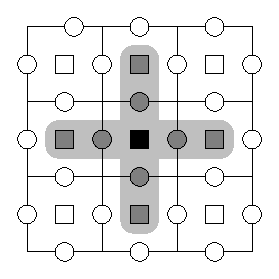
\epsfig{file=fig/stencil.eps,width=1.5in}
\end{minipage} 
\end{center}

First we integrate over the $h_x \times h_y \times h_z$ cell $\vol$
centered at $r$, and apply the divergence rule:

 \begin{eqnarray*}
 \nabla\cdot(\ac \nabla \uc) & = & \fc \\
 \int_\vol \nabla\cdot(\av \nabla \uv)\, d\volel & = & \int_\vol \fv\, d\volel \\
 \oint_{\surf} \as \nabla \us\cdot \norm \, d\surfel & = & \int_\vol \fv\, d\volel
 \end{eqnarray*}

Next we break up the surface integral over the cell surface $\surf$
into separate integrals over each of the six cell faces
$\sidexp,\sidexm,\sideyp,\sideym,\sidezp$ and $\sidezm$:

 \begin{eqnarray*}
 \oint_{\sidexp} \as \nabla \us\cdot \norm \, d\surfel +  \oint_{\sidexm} \as \nabla \us\cdot \norm \, d\surfel & + & \\
 \oint_{\sideyp} \as \nabla \us\cdot \norm \, d\surfel +  \oint_{\sideym} \as \nabla \us\cdot \norm \, d\surfel & + & \\
 \oint_{\sidezp} \as \nabla \us\cdot \norm \, d\surfel +  \oint_{\sidezm} \as \nabla \us\cdot \norm \, d\surfel & = & \int_\vol \fv\, d\volel
 \end{eqnarray*}

Next we approximate the surface and volume integrals using the
midpoint rule, and approximate the derivatives using a centered difference:

 \begin{eqnarray*}
 |\sidexp| \axph \frac{du}{dx}(r+h_x/2) + 
 |\sidexm| \axmh \frac{du}{dx}(r-h_x/2) & + & \\ 
 |\sideyp| \ayph \frac{du}{dy}(r+h_y/2) +
 |\sideym| \aymh \frac{du}{dy}(r-h_y/2) & + & \\ 
 |\sidezp| \azph \frac{du}{dz}(r+h_z/2) + 
 |\sidezm| \azmh \frac{du}{dz}(r-h_z/2) & = & |\vol| \fc  \\
\\
 h_y h_z \axph \frac{du}{dx}(r+h_x/2) + 
 h_y h_z \axmh \frac{du}{dx}(r-h_x/2) & + & \\ 
 h_z h_x \ayph \frac{du}{dy}(r+h_y/2) +
 h_z h_x \aymh \frac{du}{dy}(r-h_y/2) & + & \\ 
 h_x h_y \azph \frac{du}{dz}(r+h_z/2) + 
 h_x h_y \azmh \frac{du}{dz}(r-h_z/2) & = & h_xh_yh_z \fc  \\
\\
 \frac{h_y h_z}{h_x} [\axph (u(r+h_x) - u(r))  + 
                      \axmh (u(r-h_x) - u(r))] & + & \\ 
 \frac{h_z h_x}{h_y} [\ayph (u(r+h_y) - u(r))  + 
                      \aymh (u(r-h_y) - u(r))] & + & \\ 
 \frac{h_x h_y}{h_z} [\azph (u(r+h_z) - u(r))  + 
                      \azmh (u(r-h_z) - u(r))] & = &  h_xh_yh_z \fc  \\
\\
 \alxp (\Uxp - \Uc)  + 
 \alyp (\Uyp - \Uc)  + 
 \alzp (\Uzp - \Uc) & + & \\ 
 \alxm (\Uxm - \Uc)  + 
 \alym (\Uym - \Uc)  + 
 \alzm (\Uzm - \Uc) & = &  F  \\
 \end{eqnarray*}

where

\[\alxm  \equiv  \frac{h_yh_z}{h_x} \axmh,
 \alym  \equiv  \frac{h_zh_x}{h_y} \aymh, 
 \alzm  \equiv  \frac{h_xh_y}{h_z} \azmh \]
 \[\alxp  \equiv  \frac{h_yh_z}{h_x} \axph, 
 \alyp  \equiv  \frac{h_zh_x}{h_y} \ayph,
 \alzp  \equiv  \frac{h_xh_y}{h_z} \azph \]
 \[F = h_xh_yh_z f(r). \]

If we assume $a(x)\equiv 1$ (Poisson equation), $h\equiv h_x = h_y =
h_z$, and if we scale $\nabla\cdot(\ac \nabla \uc) = f$ by multiplying
each side by $C_h \equiv 1/h$, then we have

\[ \Uxp + \Uyp + \Uzp - 6\Uc + \Uxm + \Uym + \Uzm = h^2 \fc \]

%-----------------------------------------------------------------------
\subsection{Discretization between grid patches} \label{ss:discret-amr}
%-----------------------------------------------------------------------

All inter-level discretizations involve zones along a patch boundary;
however, not all zones along a patch boundary are involved in
inter-level discretization.  Since we will be discussing zones along a
patch boundary, we define a zone to be a ``\textit{face-zone}'' if it
lies along the external boundary of its containing grid patch.


%-----------------------------------------------------------------------
\subsubsection{Face-zone categorization}
%-----------------------------------------------------------------------

Face zones are assigned to one of the five categories listed below.
Note that ``neighbor'' implies ``in the same refinement level'',
whereas ``adjacent'' does not.


\begin{minipage}{1in}
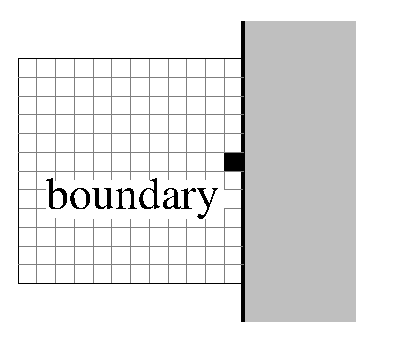
\epsfig{file=fig/neighbor-boundary.eps,width=1in}
\end{minipage} \
\begin{minipage}{5.8in}
 A \textbf{boundary face-zone} is adjacent to the domain boundary.  We
assume boundary face-zones are always in the coarsest grid level; and
if one face-zone along a grid face is a boundary face-zone, then all
face-zones in that face are boundary face-zones
\end{minipage}

\begin{minipage}{1in}
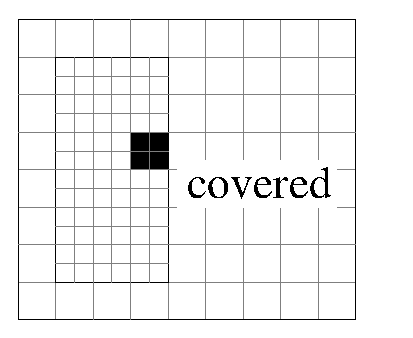
\epsfig{file=fig/neighbor-covered.eps,width=1in}
\end{minipage} \
\begin{minipage}{5.8in}
A \textbf{covered face-zone} is covered by face zones in a finer
level.  Each grid that contains a covered face-zone contains a child
grid that covers the zone.
\end{minipage}

\begin{minipage}{1in}
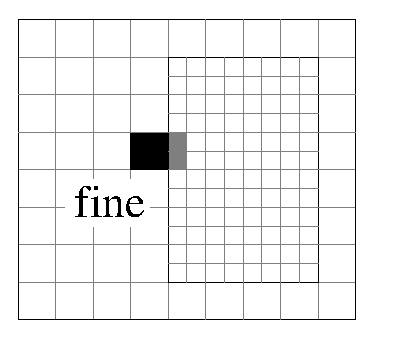
\epsfig{file=fig/neighbor-fine.eps,width=1in}
\end{minipage} \
\begin{minipage}{5.8in}
A \textbf{fine face-zone} is adjacent to zones in a child of a
neighbor of the containing patch's parent.  Each fine face-zone is not
covered, its containing grid has a neighboring grid adjacent to the
face-zone, and the paired face-zone in the neigboring grid is covered.
We assume that all adjacent zones must not span more than one level.
\end{minipage}


\begin{minipage}{1in}
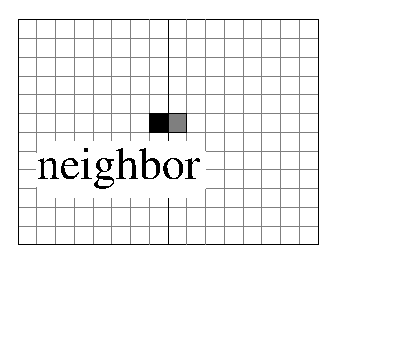
\epsfig{file=fig/neighbor-neighbor.eps,width=1in}
\end{minipage} \
\begin{minipage}{5.8in}
A \textbf{neighbor face-zone} is adjacent to a zone in a neighboring
patch.  The neighboring patch and containing patch may not necessarily
have the same parent.  Each neighbor face-zone is not covered, the
containing grid has a neighboring grid adjacent to the face-zone, and
the paired face-zone in the neighboring grid is not covered.
\end{minipage}

\begin{minipage}{1in}
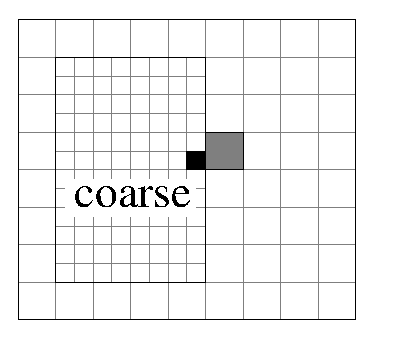
\epsfig{file=fig/neighbor-coarse.eps,width=1in}
\end{minipage} \
\begin{minipage}{5.8in}
A \textbf{coarse face-zone} is adjacent to a zone in the containing
patch's parent, or a zone in a neighbor of the containing patch's
parent.  Each coars face-zone is not covered, and the containing grid
does not have a neighboring grid adjacent to the face-zone.  We assume
that all adjacent zones must not be more than one level apart.
\end{minipage}


We use these characteristics to derive algorithms for categorizing
face-zones.  While we don't need to know all categories (only coarse,
fine, and boundary face-zones are used), some categories are easier to
determine if other categories are known.  In particular, our algorithm
for categorizing coarse face-zones is to categorize all other
face-zones, and all uncategorized face-zones are then categorized as
coarse.

\begin{center}
\begin{tabular}{l|cccc}
category & boundary & covered & adjacent grid & covered neighbor \\ \hline
boundary & true &  \\
covered  &        & true \\
fine     & false & false & true & true \\
neighbor & false & false  & true& false \\
coarse   & false & false  & false \\
\end{tabular}
\end{center}

Categorizing requires four phases:

\begin{itemize}
\item[1.] Categorize boundary face-zones
\begin{tabbing}
xxx\=xxx\=xxx\=xxx\=xxx\=xxx\=xxx\=xxxxxxxxxxxxxxxxxxx\=\kill
\> \textbf{for} \code{grid} in \code{level(0)} \\
\>\> \textbf{for} \code{face} in \code{grid} \\
\>\>\> \textbf{if} \code{face} along boundary \\
\>\>\>\> \textbf{for} \code{face-zone} in \code{face} \\
\>\>\>\>\> \code{categorize (face-zone , BOUNDARY)}
\end{tabbing}
\item[2.] Categorize covered face-zones
\begin{tabbing}
xxx\=xxx\=xxx\=xxx\=xxx\=xxx\=xxx\=xxxxxxxxxxxxxxxxxxx\=\kill
\> \textbf{for} \code{level} in \code{hierarchy} (fine to next-coarsest) \\
\>\> \textbf{for} \code{grid} in \code{level} \\
\>\>\> \code{sub-face = intersection (grid.face , parent(grid).face)} \\
\>\>\>\> \textbf{for} \code{face-zone} in \code{sub-face} of \code{parent(grid)}\\
\>\>\>\>\>     \code{categorize (face-zone , COVERED)} \\
\>\>\>\> \textbf{for} \code{face-zone} in \code{sub-face} of \code{adjacent(parent(grid))}\\
\>\>\>\>\>     \textbf{if} \code{face-zone not covered} \\
\>\>\>\>\>\> \code{categorize (face-zone , ADJACENT-COVERED)}
\end{tabbing}
\item[3.] Categorize fine and neighbor face-zones
\begin{tabbing}
xxx\=xxx\=xxx\=xxx\=xxx\=xxx\=xxx\=xxxxxxxxxxxxxxxxxxx\=\kill
\> \textbf{for} \code{level} in \code{hierarchy} (fine to coarse) \\
\>\> \textbf{for} \code{grid} in \code{level} \\
\>\>\> \textbf{for} \code{neighbor} of \code{grid} \\
\>\>\>\> \code{sub-face = intersection (grid.face , neighbor.face)} \\
\>\>\>\> \textbf{for} \code{face-zone} in \code{sub-face} of \code{grid}\\
\>\>\>\>\> \textbf{if} \code{face-zone is adjacent-covered} \\
\>\>\>\>\>\> \code{categorize (face-zone , FINE)} \\
\>\>\>\>\> \textbf{else if} \code{face-zone is not covered} \\
\>\>\>\>\>\> \code{categorize (face-zone , NEIGHBOR)}
\end{tabbing}
\item[4.] Categorize coarse face-zones
\begin{tabbing}
xxx\=xxx\=xxx\=xxx\=xxx\=xxx\=xxx\=xxxxxxxxxxxxxxxxxxx\=\kill
\> \textbf{for} \code{face-zone} in \code{hierarchy} \\
\>\> \textbf{if} \code{face-zone} not categorizeed \\
\>\>\>        \code{categorize (face-zone , COARSE)}
\end{tabbing}
\end{itemize}


%-----------------------------------------------------------------------
\subsubsection{Face-zone discretization}
%-----------------------------------------------------------------------

By default, zone connections are defined using stencil connections defined
using \hypre\ stencil values, which we derive in \S\ref{ss:discret-unigrid}.
Below, we derive modifications for each category of face-zone.


\begin{minipage}{1.75in}
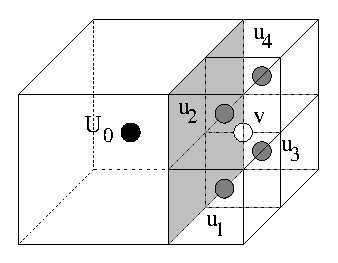
\epsfig{file=fig/discret-coarse-4.eps,width=1.5in} % width 2in
\end{minipage} \ \ \ \ 
\begin{minipage}{4.00in}
\begin{eqnarray*}
& \oint_{\sideXP}  \!\!\! & \as \nabla \us\cdot \norm \, d\surfel  \\
& \approx & |\sideXP| \axpH \frac{v - U_0}{\frac{3}{4}H_x} \\
& = & \frac{H_yH_z}{H_x} \axpH \frac{4}{3} (\frac{1}{4} \sum_{k=1}^4 u_k - U_0)   \\
\end{eqnarray*}
\end{minipage}


\begin{minipage}{1.75in}
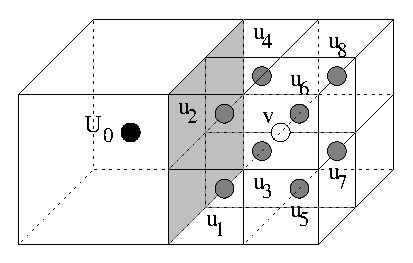
\epsfig{file=fig/discret-coarse-8.eps,width=1.875in} % width 2.5in
\end{minipage} \ \ \ \ 
\begin{minipage}{4.00in}
\begin{eqnarray*}
& \oint_{\sideXP} \!\!\! & \as \nabla \us\cdot \norm \, d\surfel  \\
& \approx & |\sideXP| \axpH \frac{v - U_0}{H_x} \\
& = & \frac{H_yH_z}{H_x}  \axpH (\frac{1}{8} \sum_{k=1}^8 u_k - U_0)   \\
\end{eqnarray*}
\end{minipage}

\begin{minipage}{1.75in}
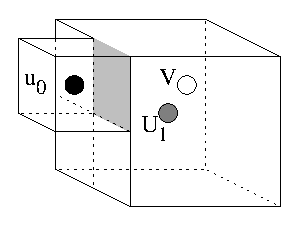
\epsfig{file=fig/discret-fine-1.eps,width=1.3125in}  % width 1.75in
\end{minipage} \ \ \ \ 
\begin{minipage}{4.00in}
\begin{eqnarray*}
& \oint_{\sidexp} \!\!\! & \as \nabla \us\cdot \norm \, d\surfel  \\
& \approx & |\sidexp| \axph \frac{V - u_0}{\frac{3}{2}h_x} \\
& = & \frac{h_yh_z}{h_x}  \axph \frac{2}{3} (U_1 - u_0)   \\
\end{eqnarray*}
\end{minipage}

\begin{minipage}{1.75in}
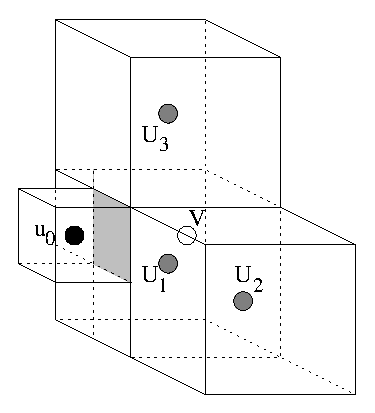
\epsfig{file=fig/discret-fine-3.eps,width=1.6875in}   % width 2.25in
\end{minipage} \ \ \ \ 
\begin{minipage}{4.00in}
\begin{eqnarray*}
& \oint_{\sidexp}  \!\!\! & \as \nabla \us\cdot \norm \, d\surfel  \\
& \approx & |\sidexp| \axph \frac{V - u_0}{\frac{3}{2}h_x} \\
& = & \frac{h_yh_z}{h_x}  \axph \frac{2}{3} (\frac{1}{2}U_1 + \frac{1}{4}U_2 + \frac{1}{4}U_3 - u_0)   \\
\end{eqnarray*}
\end{minipage}


\begin{minipage}{1.75in}
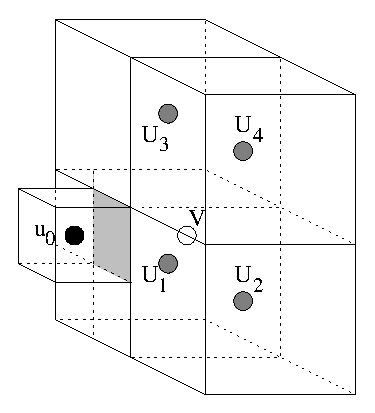
\epsfig{file=fig/discret-fine-4.eps,width=1.6875in}   % width 2.25in
\end{minipage} \ \ \ \ 
\begin{minipage}{4.00in}
\begin{eqnarray*}
& \oint_{\sidexp}  \!\!\! & \as \nabla \us\cdot \norm \, d\surfel \\
& \approx & |\sidexp| \axph \frac{V - u_0}{\frac{3}{2}h_x} \\
& = & \frac{h_yh_z}{h_x}  \axph \frac{2}{3} (\frac{9}{16} U_1 + \frac{3}{16} U_2 + \frac{3}{16} U_3 + \frac{1}{16}U_4 - u_0)   \\
\end{eqnarray*}
\end{minipage}


\begin{minipage}{1.75in}
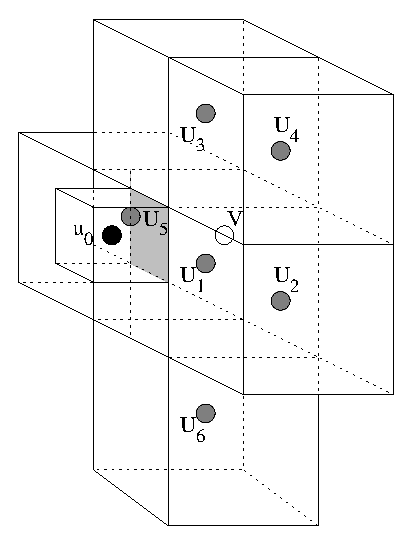
\epsfig{file=fig/discret-fine-6.eps,width=1.875in}    % width 2.50in
\end{minipage} \ \ \ \ 
\begin{minipage}{4.00in}
\begin{eqnarray*}
 & \oint_{\sidexp} \!\!\! & \as \nabla \us\cdot \norm \, d\surfel  \\
 & \approx & |\sidexp| \axph \frac{V - u_0}{\frac{3}{2}h_x} \\
& = & \frac{h_yh_z}{h_x}  \axph \frac{2}{3} (\frac{30}{32} U_1 + \frac{3}{32} U_2 + \frac{3}{32} U_3 + \frac{2}{32}U_4 - \frac{3}{32}U_5 - \frac{3}{32}U_6 - u_0)   \\
\end{eqnarray*}
\end{minipage}


%\begin{center}
%\begin{minipage}{1.25in}
%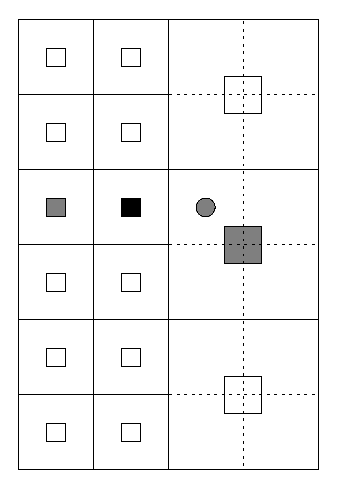
\epsfig{file=fig/stencil0.eps,width=1.25in} \\
%\centerline{Piecewise constant}
%\end{minipage} \ \ \ 
%\begin{minipage}{1.25in}
%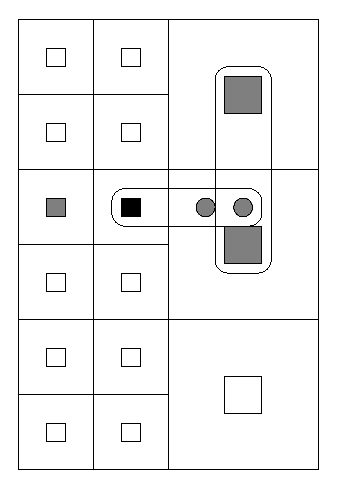
\epsfig{file=fig/stencil1.eps,width=1.25in} \\
%\centerline{Piecewise linear}
%\end{minipage} \ \ \ 
%\begin{minipage}{1.25in}
%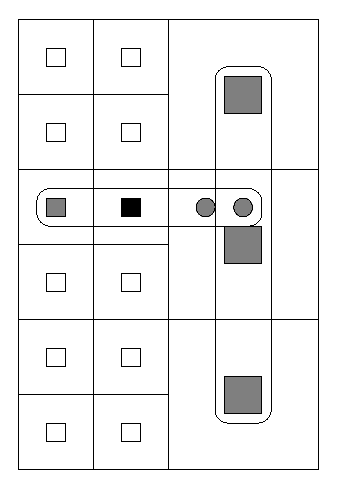
\epsfig{file=fig/stencil2.eps,width=1.25in} \\
%\centerline{Piecewise quadratic}
%\end{minipage}
%\end{center}


% \begin{center}
% \begin{minipage}{6.0in}
% 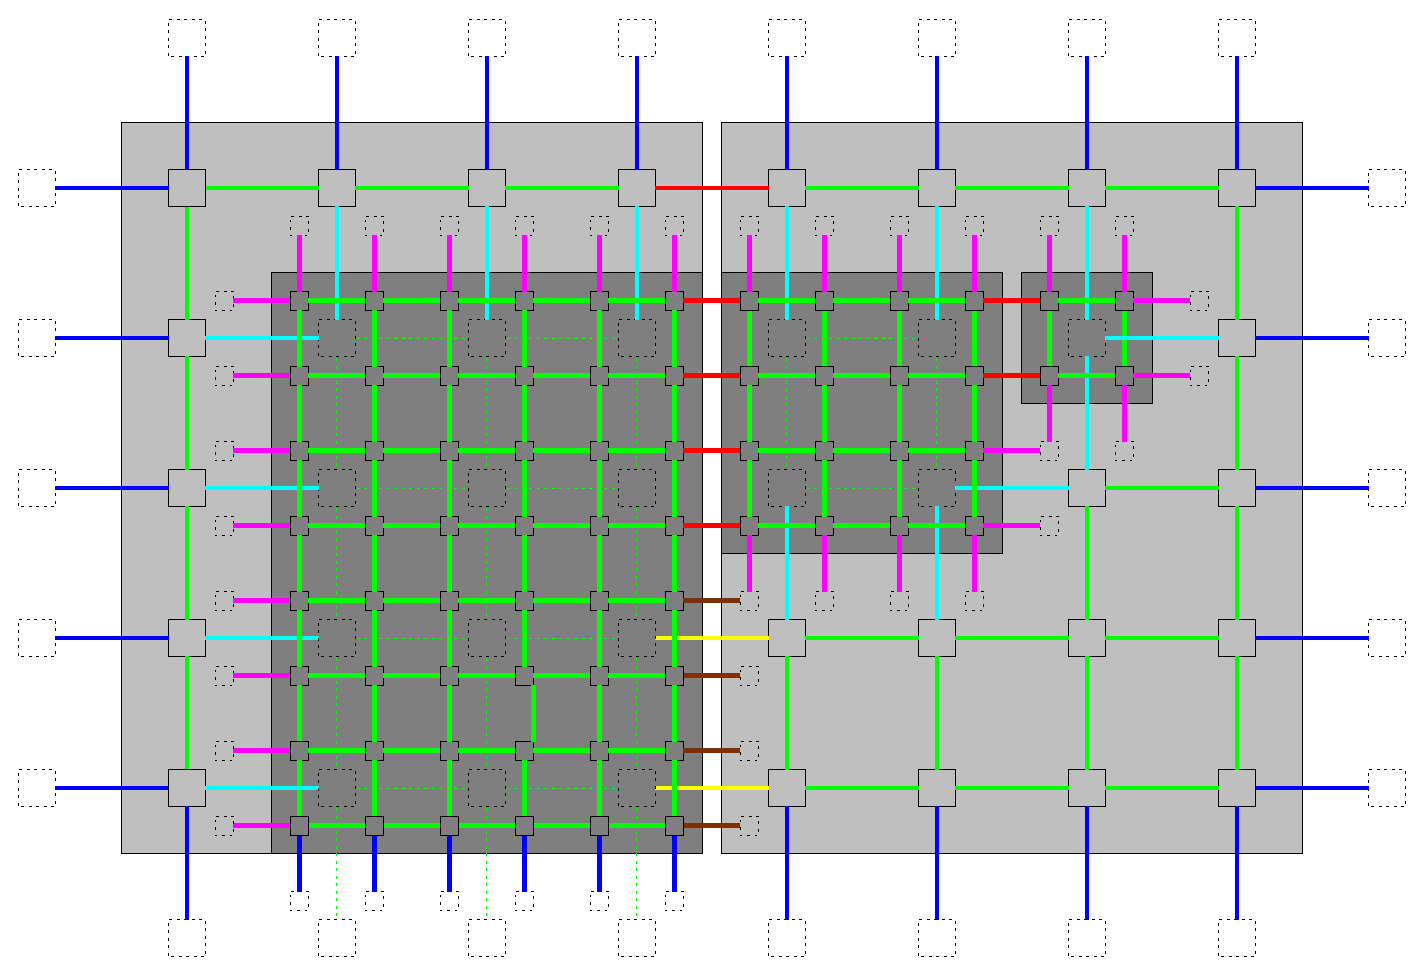
\epsfig{file=fig/discret-step-1.eps,width=6.0in}
% \end{minipage}
% \end{center}

% Types of matrix elements for a given unknown:
% 
% \begin{tabular}{ll}
% \textcolor{green}{internal} & \code{HYPRE\_SStructStencilSetEntry()} \\
% \textcolor{green}{overlapped internal} & \code{HYPRE\_SStructStencil} \\
% \textcolor{red}{neighbor} & \code{HYPRE\_SStructGridSetNeighborBox()}\\
% \textcolor{blue}{boundary} & \code{HYPRE\_SStructGraphAddEntries()}\\
% \textcolor{magenta}{fine-coarse parent} & \code{HYPRE\_SStructGraphAddEntries()}\\
% \textcolor{cyan}{coarse-fine child} & \code{HYPRE\_SStructGraphAddEntries()}\\
% \textcolor{brown}{fine-coarse parent--neighbor} & \code{HYPRE\_SStructGraphAddEntries()}\\
% \textcolor{yellow}{coarse-fine neighbor--child} & \code{HYPRE\_SStructGraphAddEntries()}\\
% \end{tabular}

%-----------------------------------------------------------------------
\subsection{Boundary Discretization} \label{ss:discret-boundary}
%-----------------------------------------------------------------------

%=======================================================================
\section{Porting to \enzo}
%=======================================================================

%=======================================================================
\section{Test Results} \label{s:results}
%=======================================================================

\begin{itemize}
\item Accuracy
\item Performance
\item Scaling
\item Robustness
\end{itemize}


\begin{tabular}{l|l} \\
\textbf{Term} & \textbf{Term description} \\ \hline
$N_0$ & Root-grid zones per processor \\
$n_0$ & Root-grid zones-per-axis  per processor \\
$N_P$ & Number of processors \\
$N_G$ & Number of grids \\
$N_L$ & Number of levels \\
$N_Z$ & Number of zones \\
\end{tabular}

\begin{tabular}{l|ccccc} \\
Problem & $N_0$ & $N_P$ & $N_G$ & $N_L$ & $N_Z$ \\ \hline
serial-unigrid       & $8^3:\sqrt{2}:128^3$ & & & \\
parallel-unigrid     & $16^3:2\ldots 128^3$ & & & \\
Simple serial AMR    & $32^3\ldots 128^3$ & & & \\
Simple parallel AMR  & $32^3\ldots 128^3$ & & & \\
General serial AMR   & $32^3\ldots 128^3$ & & & \\
General parallel AMR & $32^3\ldots 128^3$ & & & \\
Large AMR            & $32^3\ldots 128^3$ & & & \\
\end{tabular}

\begin{tabular}{l|l} \\
\textbf{Plot name} & \textbf{Plot description} \\ \hline
\code{procs-mem} & Processor count versus memory (bytes) \\
\code{procs-mem-zone} & Processor count versus memory per zone (bytes) \\
\code{procs-time} & Processor count versus time (seconds) \\
\code{procs-time-zone} & Processor count versus time per zone (seconds) \\
\code{size-mem-zone} &  Problem size (number of zones) versus memory per zone (bytes) \\
\code{size-mem-zone} &  Problem size ($n$) versus memory (bytes) \\
\code{size-time-zone} &  Problem size (number of zones) versus time per zone (seconds) \\
\code{size-time-zone} &  Problem size ($n$) versus time (seconds) \\
\end{tabular}

\EndDOCUMENT

\end{document}
%==================================================================

